\section{\protein{Mad1}'s loop region is important to the SAC signaling activity \Latin{in vivo}}
\label{LoopDeletionSection}

We next sought to determine whether the loop region of \protein{Mad1} that likely enables the fold-back conformation is important to the SAC signaling activity \Latin{in vivo}. We integrated the expression cassette of either \protein{Mad1}-mNG or \protein{Mad1}\textDelta{}L-mNG into the genome of HeLa-A12 cells using Cre-\bacterialgene{lox} RMCE (see \myref{Cre-lox}). We then knocked down endogenous \protein{Mad1} in these cells using two siRNAs that target the 3'-UTR of \gene{Mad1} \cite{siMAD1-3UTR} (henceforth collectively referred to as si\gene{Mad1}'s) and induced the expression of \protein{Mad1}(WT/\textDelta{}L)-mNG (si\gene{Mad1}-resistant due to the lack of the endogenous 3'-UTR) by doxycycline. Our genome-edited \gene{Mad1}-mNG HeLa-A12 cell line served as the reference for the endogenous level of \protein{Mad1} in live-cell fluorescence imaging.

We found out that knocking down \gene{Mad1} crippled the SAC signaling activity (see \myref{MAD1Rescue_Main}), although cells with less than 10\% of the physiological level of \protein{Mad1} on average (estimated from the immunoblot in \myref{MAD1Rescue_WB}) still arrested in mitosis for hours when treated with \SI{100}{nM} nocodazole (only about two hours less than the control group with a physiological level of \protein{Mad1}). Increasing the dosage of si\gene{Mad1}'s did not further decrease the SAC activity, reinforcing that even a small pool of \protein{Mad1} could sustain a considerable level of SAC signaling activity (see \myref{MAD1Rescue_LimitPushing}).

\begin{figure}
    \centering
    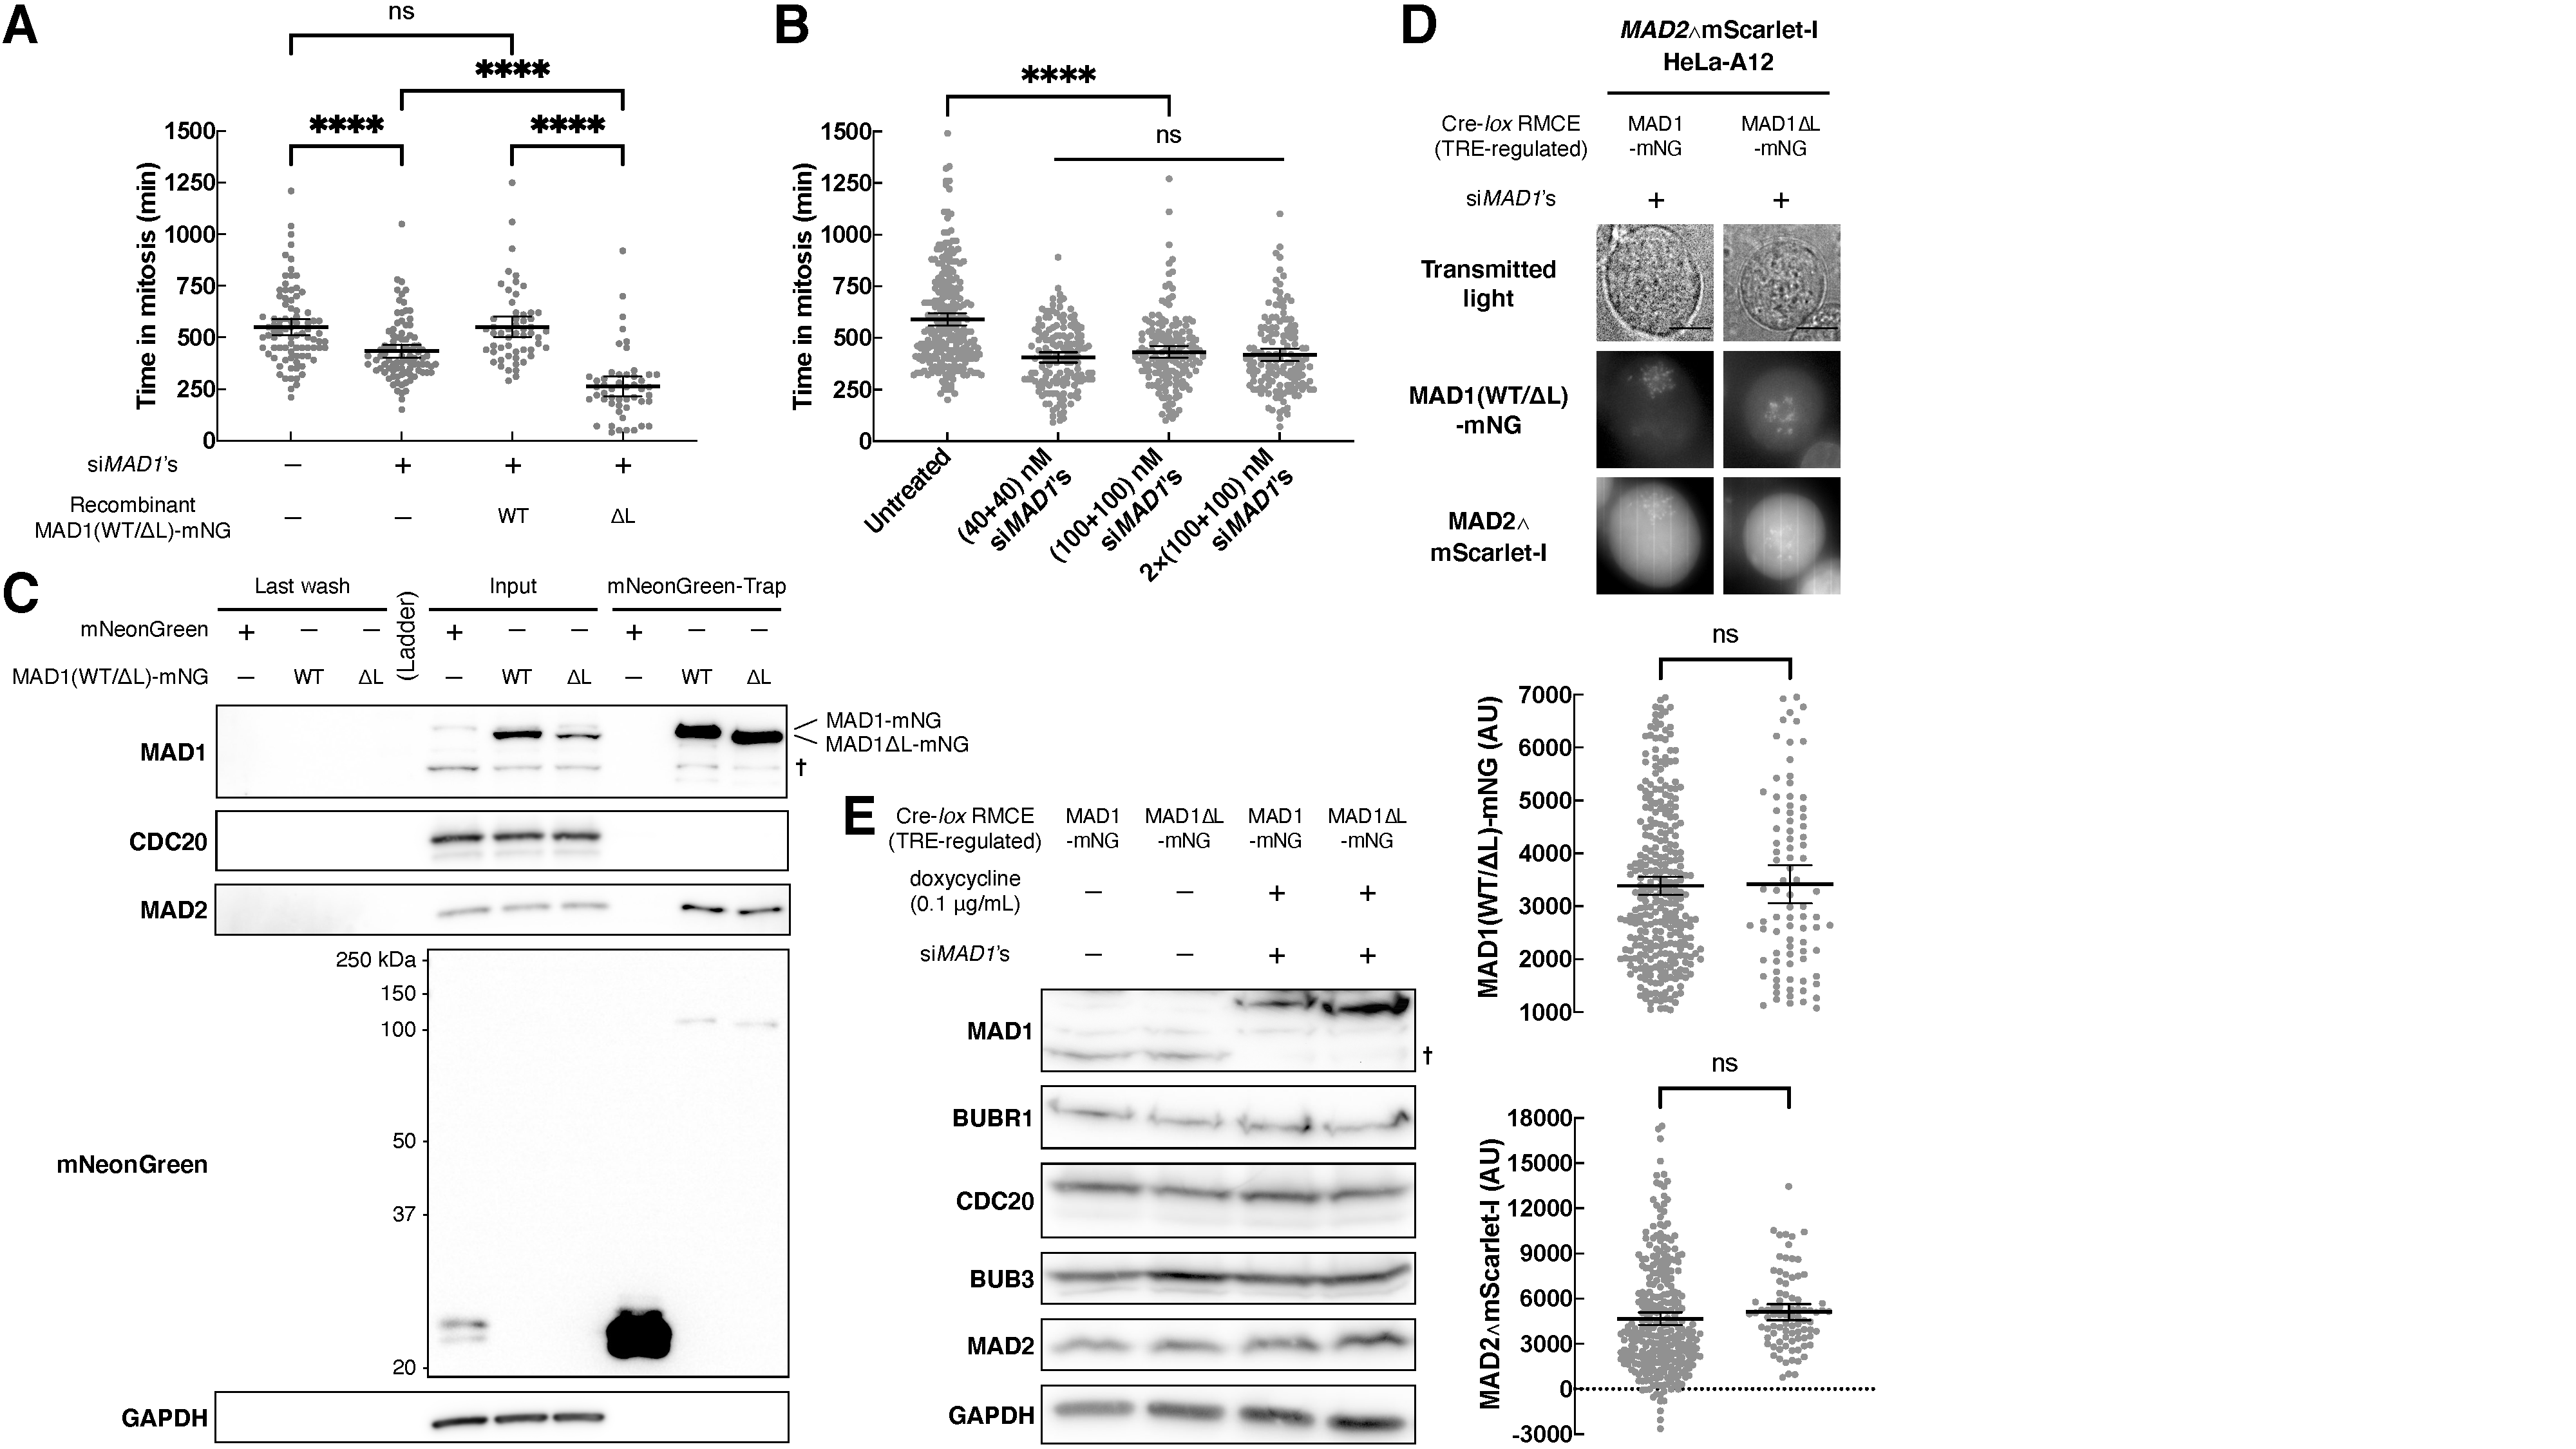
\includegraphics[trim={0 0 0 3cm},clip]{chapters/figures/MAD1Rescue.pdf}
    \phantomsubfiglabel{MAD1Rescue_Main} % subfigure A
    \phantomsubfiglabel{MAD1Rescue_LimitPushing} % subfigure B
    \phantomsubfiglabel{MAD1Rescue_HeterodimerizationWB} % subfigure C
    \phantomsubfiglabel{MAD1Rescue_Localization} % subfigure D
    \phantomsubfiglabel{MAD1Rescue_WB} % subfigure E
    \caption{\textbf{The loop region of \protein{Mad1} is critical to the SAC signaling activity in its own right.}}
    \label{MAD1Rescue}
\end{figure}
\begin{figure}
    \noindent\justifying \textbf{(Caption of \myref{MAD1Rescue} continued from a previous page)} (A) The two columns on the left used the \gene{Mad1}-mNG genome-edited HeLa-A12 cell line, which served as a reference of the endogenous level of \gene{Mad1} (si\gene{Mad1}'s which target the 3'-UTR of \gene{Mad1} are effective against \gene{Mad1}-mNG here as confirmed by the greatly diminished green channel fluorescence signal). The two columns on the right were from the Cre-\bacterialgene{lox} RMCE HeLa-A12 cell line. Each dot represents a cell ($N \geq 50$ in each group). Results were pooled from at least two technical repeats. The mean value $\pm$ the 95\% confidence interval of each group is overlaid. Unpaired $t$-tests with Welch's correction were performed in Prism 9. (B) The conditions of si\gene{Mad1} treatment were (from left to right): untreated, \SI{40}{nM} each for two days (the standard condition used throughout this study), \SI{100}{nM} each for two days, \SI{100}{nM} each in day one and \SI{100}{nM} each again in day two. The \gene{Mad1}-mNG genome-edited HeLa-A12 cell line was used in each group. Each dot represents a cell ($N \geq 145$ in each group). The mean value $\pm$ the 95\% confidence interval of each group is overlaid. Welch's ANOVA test [$W(\text{DF}n, \text{DF}d) = 0.9885 (2.000, 298.9)$, $p = 0.3733$] was performed for the three columns on the right. The ANOVA test and the unpaired $t$-test with Welch's correction were done in Prism 9. (C) Using immunoblotting to evaluate the immunoprecipitation by the mNeonGreen-Trap Agarose. The cruciform symbol represents the endogenous \protein{Mad1} band. The expected molecular weights of the recombinant \protein{Mad1}-mNG, \protein{Mad1}\textDelta{}L-mNG, and mNeonGreen are \SI{110.2}{kDa}, \SI{108.4}{kDa}, and \SI{26.9}{kDa}, respectively. GAPDH served as the loading control. (D) The \gene{Mad2}$\wedge$mScarlet-I genome-edited HeLa-A12 treated with si\gene{Mad1}'s and rescued by \protein{Mad1}(WT/\textDelta{}L)-mNG were imaged using wide-field, $z$-stack fluorescence microscopy. Cells were arrested at mitosis using a thymidine--nocodazole synchronization protocol. Representative micrographs are shown in the top panel. Maximum $z$-projected red channel images shown here share the same LUT (and so are the maximum $z$-projected green channel images). Scale bar, \SI{10}{\micro m}. Due to various induced expression of \protein{Mad1}(WT/\textDelta{}L)-mNG in different cells, signaling kinetochores were filtered by the localization of \protein{Mad1}(WT/\textDelta{}L)-mNG (1000--\SI{7000}{AU}). Each gray dot represents measurement of a single signaling kinetochore ($N \geq 85$ in each group). Unpaired $t$-tests with Welch's correction were performed in Prism 9. (E) Knockdown of the endogenous \protein{Mad1} by si\gene{Mad1}'s had an efficiency of over 90\% based on the intensity of the residual band. The expression level of other SAC proteins by immunoblotting. The cellular abundance of \protein{BubR1}, \protein{Cdc20}, and \protein{Bub3} were not affected. Unsynchornized Cre-\bacterialgene{lox} RMCEM HeLa-A12 cells were used.
\end{figure}

Surprisingly, \protein{Mad1}\textDelta{}L-mNG had impaired support for the SAC in a dominant-negative manner: cells treated with si\gene{Mad1}'s and rescued by a physiological level of \protein{Mad1}\textDelta{}L-mNG arrested in mitosis for a significantly shorter duration than cells which were not rescued. As a comparision, wildtype \protein{Mad1}-mNG fully restored the SAC signaling activity (see \myref{MAD1Rescue_Main}). One possible explanation was that \protein{Mad1}\textDelta{}L-mNG might dimerize with the remaining endogenous \protein{Mad1} and restrict its structural flexibility. Structural prediction of the heterodimer between wildtype \protein{Mad1} and \protein{Mad1}\textDelta{}L showed that the loop region of the wildtype copy introduced a bulge but could not enable a fold-back conformation of the heterodimer due to stiffness of the fused \textalpha{}-helices of the \protein{Mad1}\textDelta{}L counterpart (see \myref{MAD1-MAD1DeltaL_ColabFoldPrediction}). To prove this hypothesis, we pulled down doxycycline-induced \protein{Mad1}(wildtype/\textDelta{}L)-mNG from lysates of HeLa-A12 cells in which endogenous \protein{Mad1} was not knocked down. We found that endogenous \protein{Mad1} was also pulled down by both \protein{Mad1}-mNG and \protein{Mad1}\textDelta{}L-mNG, but not by mNeonGreen alone (see \myref{MAD1Rescue_HeterodimerizationWB}). We further confirmed that \protein{Mad1}\textDelta{}L-mNG did not cause defects in the localization of the \protein{Mad1}\textDelta{}L-\protein{Mad2} heterotetramer (see \myref{MAD1Rescue_Localization}) or the expression of \protein{BubR1}, \protein{Cdc20}, or \protein{Bub3} (see \myref{(see \myref{MAD1Rescue_WB})}). \Latin{In vitro} reconstitution data from our collaborators (not shown here) also suggested that truncating the loop region of \protein{Mad1} reduced the formation rate of \protein{Cdc20}-\protein{Mad2}. Therefore, although the results of our knockdown-rescue experiments were hindered by the incomplete knockdown of the endogenous \protein{Mad1}, all evidence combined suggested that the loop region of \protein{Mad1} is critical to the SAC signaling activity in its own right.